\documentclass[border=4pt]{standalone}
\usepackage{amsmath,amssymb,tikz}\usetikzlibrary{arrows.meta}
\definecolor{figB}{RGB}{31,90,166}\definecolor{figR}{RGB}{176,48,48}
\begin{document}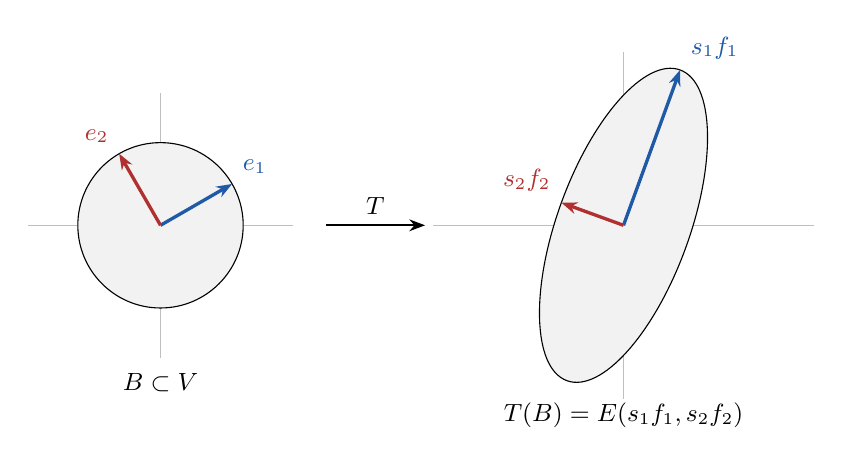
\begin{tikzpicture}[scale=1.05,>={Stealth[length=2mm]}]
\begin{scope}
\draw[gray!50] (-1.6,0)--(1.6,0) (0,-1.6)--(0,1.6);
\fill[gray!10] (0,0) circle (1); \draw (0,0) circle (1);
\draw[->,very thick,figB] (0,0)--(30:1) node[above right,font=\small]{$e_1$};
\draw[->,very thick,figR] (0,0)--(120:1) node[above left,font=\small]{$e_2$};
\node[font=\small] at (0,-1.9) {$B\subset V$};
\end{scope}
\draw[->,thick] (2.0,0)--(3.2,0) node[midway,above,font=\small]{$T$};
\begin{scope}[xshift=5.6cm]
\draw[gray!50] (-2.3,0)--(2.3,0) (0,-2.1)--(0,2.1);
\fill[gray!10,rotate=70] (0,0) ellipse (2 and 0.8); \draw[rotate=70] (0,0) ellipse (2 and 0.8);
\draw[->,very thick,figB] (0,0)--(70:2) node[above right,font=\small]{$s_1f_1$};
\draw[->,very thick,figR] (0,0)--(160:0.8) node[above left,font=\small]{$s_2f_2$};
\node[font=\small] at (0,-2.3) {$T(B)=E(s_1f_1,s_2f_2)$};
\end{scope}
\end{tikzpicture}\end{document}
